\chapter{The Telescope Signal}\label{CH1}

 The goal of an adaptive optics (AO) system is to correct for the aberrations caused by atmospheric turbulence. It is important to first understand what image we would expect on our detector for a perfectly corrected diffraction-limited system. In this chapter, we will use radiative transfer and diffraction to determine what the Intensity pattern on our detector will be from a star, and an estimate of the number of photons we can expect from a star of a given magnitude. We then describe photon noise, which affects AO system performance, and influences how the AO system is run on-sky. The point spread function (PSF) of a diffraction-limited system is then described, and we investigate how aberrations from turbulence degrade the PSF. Lastly, we describe the basic operation of an AO system and how it is used to compensate for atmospheric turbulence.

\section{Estimating the Photon Count}\label{phcount}

We model light as an electromagnetic wave, that has a characteristic complex amplitude $A$, wavelength $\lambda$, direction $\hat{a}$, and phase $\phi$. The phase is given by $\phi= \frac{2\pi}{\lambda}*OPD$, where OPD is the optical path difference. A wave with no aberrations has an OPD=0, and the phase term disappears. Light traveling from infinity, like that of stars, is described by a plane wave in Equation \ref{waveEq}. Light spans a spectrum of wavelengths that are broken up into categories based on different proprieties of the radiation at those wavelengths. The electromagnetic spectrum spans from $10^{-12}$-$m$ and smaller for gamma radiation, out to wavelengths of greater than $10^{-1}$-$m$ for radio waves. Adaptive optics systems are designed to work in the visible spectrum (380-$nm$ to 700-$nm$) out to near-infrared (700-$nm$ to 5-$\mu m$).

\begin{equation}
    U=Ae^{i(k\dot r-\omega t+ \phi)}\hat{a}
    \label{waveEq}
\end{equation}

Stars exhibit black-body radiation, which is when the power spectrum of the emitted radiation has a characteristic shape determined by the temperature of the star. We can determine the expected number of photons on our telescope primary mirror from a star by integrating Plank's Law over a wavelength bandpass. Plank's Law gives the radiant exitance $[\frac{W}{sr*m^3}]$ of electromagnetic radiation emitted by a black-body in thermal equilibrium. We need the energy per unit area radiated by black-body, or the irradiance flux density $[\frac{W}{m^2}]$. To find the flux density we integrate the radiant exitance over a wavelength range and the unit solid angle. The irradiance flux density, $I_e$ is given by,

\begin{equation}
    I_e=\int_{0}^{2pi} d\phi \int_{0}^{\frac{\pi}{2}} \cos(\theta)\sin(\theta)d\theta \int_{\lambda_{min}}^{\lambda_{max}} \frac{2hc^2}{\lambda^5}\frac{1}{exp(\frac{hc}{\lambda k_B T})-1} d\lambda
\end{equation}

where $c$ is the speed of light, $k_B$ is the Boltzmann constant, and $h$ is Planck's constant. We have now calculated the irradiance leaving the star, but we need to know the irradiance arriving on Earth. To find this we perform an intermediate step by using the irradiance flux density to calculate the luminosity of the star, $L_{\star}$ [W].

\begin{equation}
    L_{\star}=I_e*4\pi r_{star}^2
\end{equation}

The luminosity can then be used to find the irradiance from the star at Earth, which astronomers call the flux $F_{E}$.

\begin{equation}
    F_{E}=\frac{L_{\star}}{4\pi r_{E}^2}
\end{equation}

Where $r_{E}$ is the distance from the source to Earth. Typically we do not need this full calculation to find the flux. Stars are cataloged on an apparent magnitude scale. Equation \ref{magnitude} links the star's magnitude to the flux, compared to a reference star of known flux and magnitude. Vega is a common flux zero-point star, and there are look-up tables of flux values of Vega at different wavelength bandpasses. 

\begin{equation}
    m_1-m_2=
    2.5 \log\left(
        \frac{f_1}{f_2}
    \right)
    \label{magnitude}
\end{equation}

 We multiply the flux by the surface area of the primary mirror of the telescope to find the power which is defined as the collected energy per second

\begin{equation}
    P=F_{E}*\pi*r_T^2
\end{equation}

The estimated Energy [J] of a photon in the observed bandpass is given by,

\begin{equation}
    E=\frac{hc}{\lambda}
\end{equation}

where $\lambda$ is the mean wavelength in the bandpass. Dividing the power by the energy of a photon gives the number of photons incident on our telescope per second.

\begin{equation}
    N_p=\frac{P}{E}
\end{equation}

This is an ideal estimate, as it assumes all photons from the star in that bandpass reach the instrument. The actual Flux incident on the telescope includes factors to account for the transmission of Earth's atmosphere, the transmission of all the optical components in the system, and the efficiencies of reflecting optics including that of the telescope primary and secondary mirrors. 


\section{Photon Noise}

The counting of photons is a random process described by the Poisson distribution. The error on the measurement of photon count is called photon noise and is the dominant error in a pyramid wavefront sensor error budget. Suppose we are counting photons over a time $T$, in discrete intervals $dt$. The photon rate of emission by the source is $v$, in units of [photons/second]. The average number of photons counted is $<m>=T/dt * vdt=Tv$. The probability of counting $m$ number of photons in the time interval $T$ is,

\begin{equation}
    P(x)=\frac{e^{-Tv} (Tv)^m}{m!}
\end{equation}

which is the Poisson distribution. The variance of values in the Poisson distribution is $\sigma^2=m$, and the standard deviation is $\sigma=\sqrt{m}$. 

A pyramid wavefront sensor measures the wavefront error using the intensity on a detector. As the number of photons incident on the detector increases, the Poisson distribution approaches a Normal distribution via the central limit theorem. The noise on a measurement from a Poisson distribution is the square root of the total number of photons counted, $\sigma_I=\sqrt{N}.$ This uncertainty in our photon count directly corresponds to an uncertainty in the measurement of the shape and amplitude of the wavefront aberration. In the linear regime we expect the error on the measured wavefront to follow the Poisson distribution as well because we are measuring wavefront error using intensity measurements. For each wavefront sensor there is a direct relationship between the photon noise and the error on the wavefront measurement, and we quantify it using the value $\beta_p $, (\cite{guyon2005}).

\section{The Point Spread Function}

 Geometric optics describes the propagation of light as rays and assumes one point in the object is mapped to one point in the image. In geometric optics, a perfect point source object would form a perfect point image. In reality, the size of an imaged point source is finite and determined by the diffraction of light from the size, shape, and power in the aperture of our system. Diffractive optics assumes that each point in the object emits a spherical wave, and the pattern at the observation point is determined by the interference of each of those wavelets. There are approximations to the diffractive theory, and in this section, we assume the Fraunhofer approximation, which assumes the plane of observation is far from the plane of diffraction ($a^2 << \lambda z$, a= radius of aperture), and that there is a limiting aperture in the pupil plane of the optical system. The Fraunhofer equation to find a field $U_z$ given a starting field $U_0$ with aperture function $T_{ap}$ is given by equation \ref{Fraunhofer}.

\begin{equation}
U_z=\frac{e^{ikz}}{ikz}e^{i\frac{\pi (x^2+y^2)}{\lambda z}}\int_{\infty} U_0(\xi,\zeta)T_{ap}e^{\frac{-2\pi i(x\xi+y\zeta)}{\lambda z}}d\xi d\zeta
\label{Fraunhofer}
\end{equation}

The values $\xi$ and $\zeta$ are the spatial frequencies associated with the spatial coordinates x and y. The Fraunhofer diffraction equations calculate the Fourier transform of the field times the aperture function.

A light wave consists of oscillating electric and magnetic fields. In diffraction theory, we consider the propagation and diffraction of the electric field component, and refer to it simply as 'the field'. The methodology of solving diffraction problems is to start with a source, propagate the wavefront from the source to the plane of diffraction to find $U^-$, the field just before the aperture. We then solve for $U^+$ the field after the aperture and then apply Fraunhofer diffraction to find $U_z$, the field at the observation plane some far distance $z$ from the aperture. If the source is a perfect point source the field at the focal plane of the imaging system is defined as the point spread function (PSF)

To start we assume that a star is far enough away to be considered a point source. Point sources emit spherical waves, but a point source at infinity results in a plane wave given by $U^-$ when it reaches the aperture.The telescope aperture is the diffractive plane in the system and can be modeled as a circular binary mask. The electric field after diffraction through the aperture is $U^+$ and is propagated to find the electric field at the image plane $U_z$. A diagram of this set up is given in Figure \ref{fig:propagation}. 

\begin{figure}
    \centering
    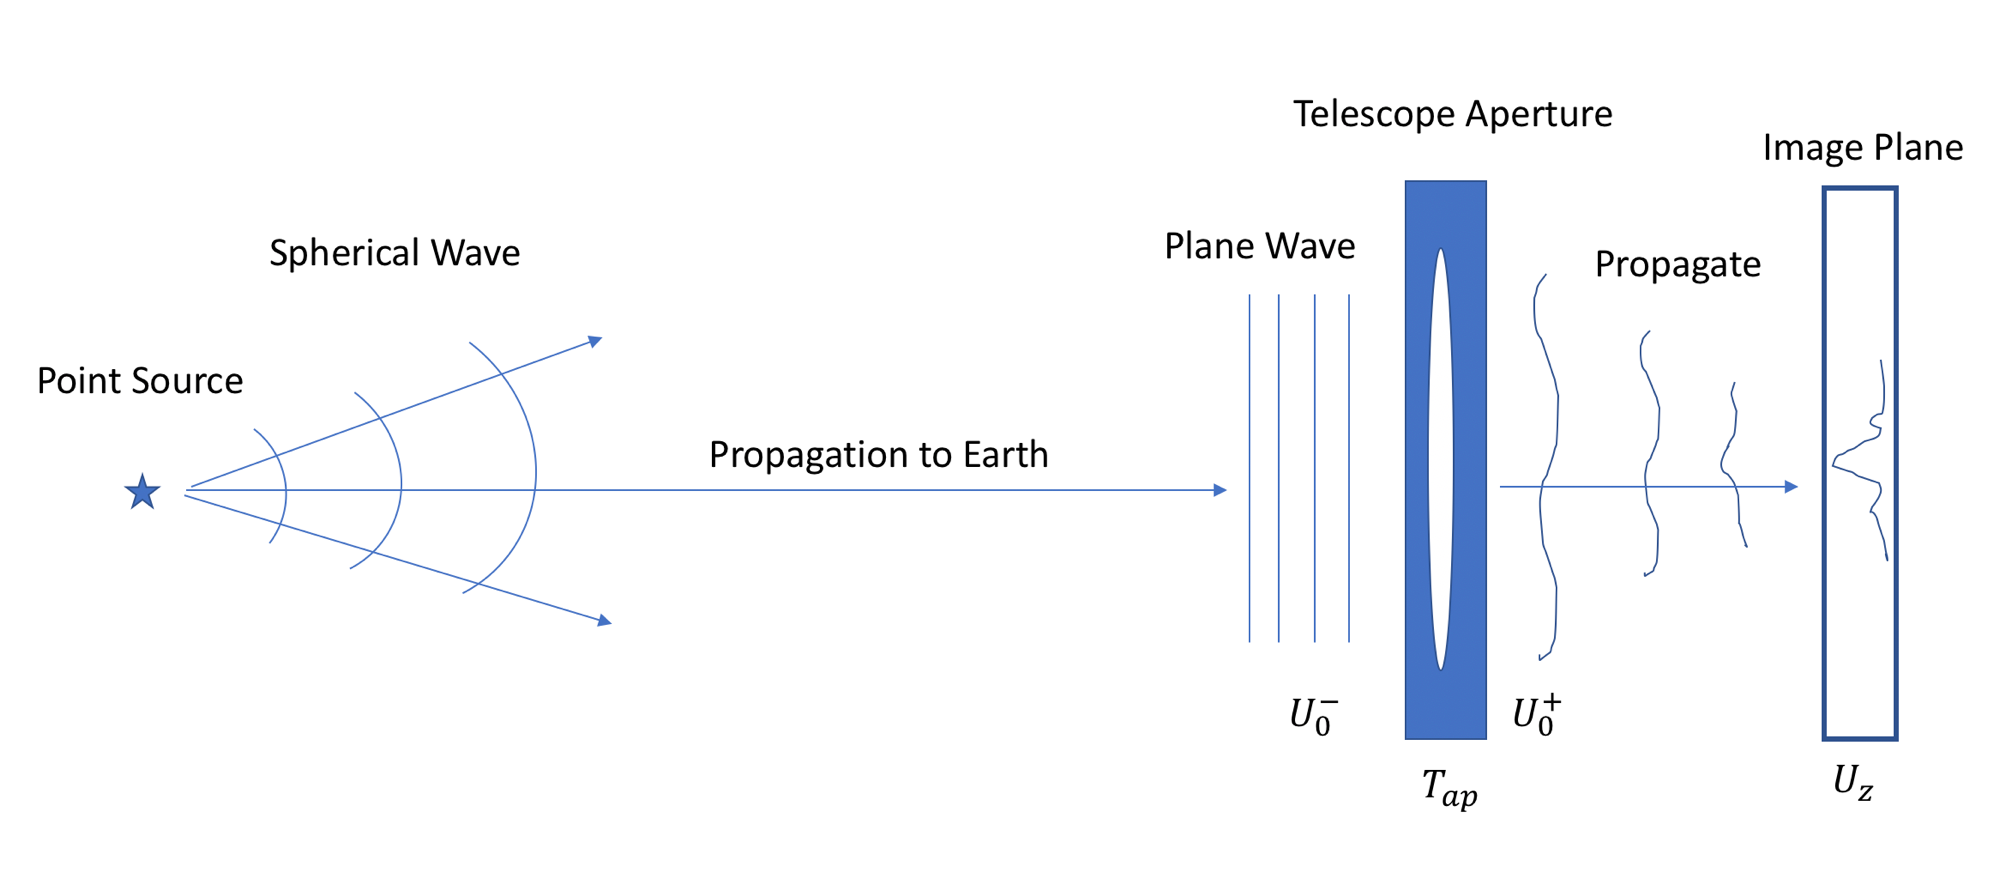
\includegraphics[width=0.75\textwidth]{Chapter Materials/Introduction Materials/Introduction Figures/Propagation.png}
    \caption{Propagation of light through an optical system. A point source at infinity results in a plane wave given by $U^-$ when it reaches the aperture. The electric field after light diffracts through the aperture is $U^+$ and is propagated to find the electric field at the image plane, $U_z$.}
    \label{fig:propagation}
\end{figure}

$U_0^-$ is modeled as a perfect plane wave in this system. For a plane was A=1 and $\phi =0$, which results in $U_0^-=1$. The PSF is then the Fourier Transform of the aperture function. The aperture function of a telescope is modeled by a circle function with diameter D, $circ(\frac{\sqrt{x^2+y^2}}{D})$, which by has a known Fourier transform that can be solved for by defining $r=\sqrt{x^2+y^2}$ and $\rho=\frac{r}{\lambda z}$. The Fourier Transform of a circ function is:

% \begin{equation}
%     h_i(x_i)= \mathcal{F}^{-1}[H_f(\xi_f)] =
%     % \frac{1}{2\pi} \int_{-\infty}^\infty e^{ i x \xi_f}
%     % \left(
%     %     \frac{1}{2} + \frac{1}{2} \mathrm{sgn}(\xi_f)
%     % \right) d\xi_f
%     % = 
%     \frac{1}{2} \delta(-x_i) + \frac{i}{2\pi} \left(\frac{1}{x_i}\right)
% \label{delta}
% \end{equation}


\begin{equation}
    \mathcal{F}\left(circ\left(\frac{r}{D/2}\right)\right)=\pi{\left(\frac{D}{2}\right)}^2 \frac{J_1(\pi D \rho)}{\frac{D\rho}{2}}
\end{equation}

which is a sombrero function. The Fraunhofer diffraction of a plane wave through a circular aperture is, 

% \begin{eqnarray}
%     S_x=\frac{I_1+I_2-I_3-I_4}{I_1+I_2+I_3+I_4}     \label{4PWFSslopes} \\
%     S_y=\frac{I_1-I_2-I_3+I_4}{I_1+I_2+I_3+I_4} \nonumber
% \end{eqnarray}

\begin{eqnarray}
   U_z=A\left(\frac{e^{ikz}}{ikz}\right)\left(e^{i\frac{\pi r^2}{\lambda z}}\right)\int_{\infty} Circ\left(\frac{r}{D/2}\right)e^{\frac{-2\pi i (r \rho )}{\lambda z}}rdrd\phi= \\
   \left(\frac{e^{ikz}}{ikz}\right)\left(e^{i\frac{\pi r^2}{\lambda z}}\right) {\left(\frac{\pi D}{2}\right)}^2 \frac{J_1 (\frac{\pi Dr}{\lambda z})}{\frac{Dr}{2\lambda z}} \nonumber
\end{eqnarray}

or,

\begin{equation}
    U_z=A \left(\frac{e^{ikz}}{ikz}\right)\left(e^{i\frac{\pi r^2}{\lambda z}}\right) {\left(\frac{\pi D}{2}\right)}^2 somb\left(\frac{2r}{\lambda z}\right)
\end{equation} 

The intensity is the modulus squared of the field,

\begin{equation}
    I(r)=A^2 {\pi^2\left(\frac{D}{2}\right)}^4 somb^2\left(\frac{2r}{\lambda z}\right)
\end{equation}

which is the Airy pattern. For more complicated apertures the PSF can be calculated in simulation by modeling the aperture as a binary mask and taking the 2D Fourier transform. The simulation can also include the calculations from Section \ref{phcount} by setting the sum of the intensity in the image to the estimated number of photons. Figure \ref{fig:Airy} shows the simulated Airy pattern for a circular aperture,

\begin{figure}
    \centering
    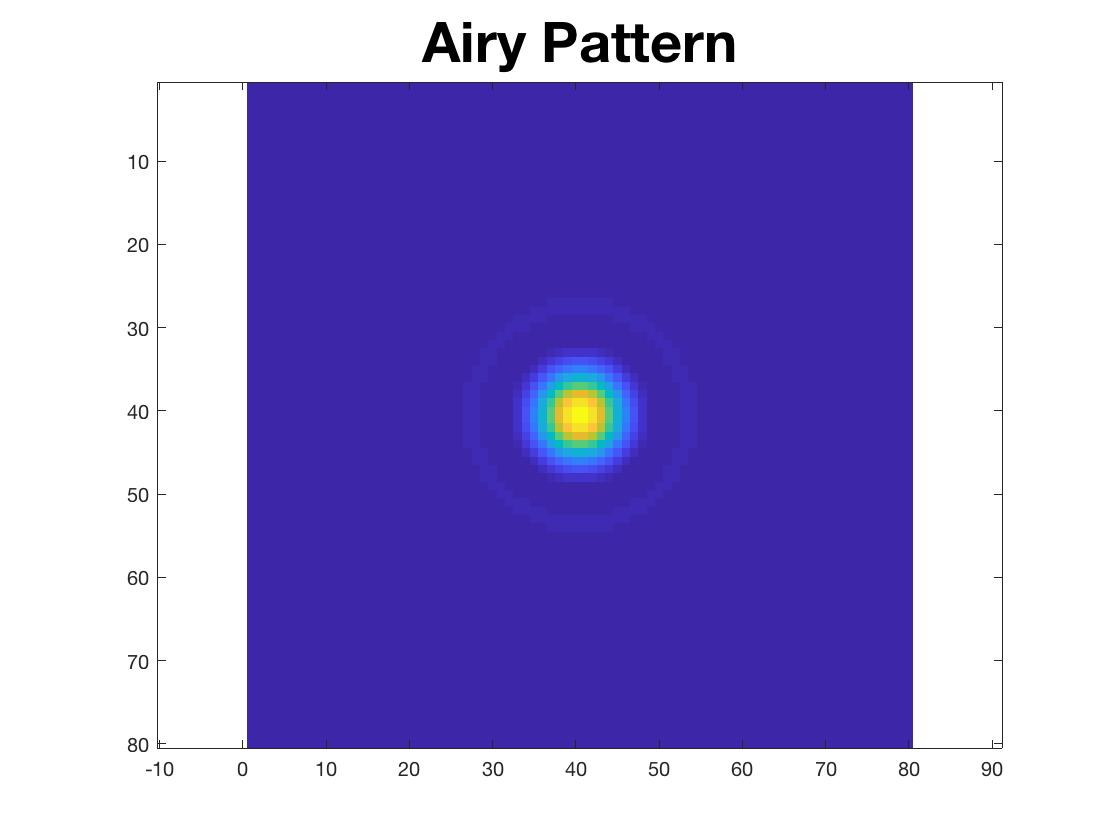
\includegraphics[width=0.5\textwidth]{Chapter Materials/Chapter One Materials/AiryPattern.jpg}
    \caption{Airy pattern generated in simulation from the diffraction of a circular aperture.}
    \label{fig:Airy}
\end{figure}

The PSF constrains the angular resolution of the imaging system which is defined in Equation \ref{res}.

\begin{equation}
    \theta=\frac{\lambda}{D}
    \label{res}
\end{equation}
 
Two objects are considered resolved if they are at least $\frac{ \lambda}{D}$ in separation. To find the physical spot size on a detector we multiply by the effective focal length.

\begin{equation}
S=\frac{ \lambda F}{D} = \lambda F_\#
\end{equation}

\subsection{Aberrations}

Aberrations degrade the image quality of an optical system. They can arise from imperfect manufacturing of optics, misalignment in the optical system, and turbulence from the atmosphere. The Optical Path Difference (OPD) is the deviation of the wavefront from a perfect reference which is illustrated in Figure \ref{fig:OPD}. OPD is measured in units of length and is related to the wavefront error that has units of radians by:

\begin{equation}
    \sigma= \frac{2\pi OPD}{\lambda}.
\end{equation}

The OPD can be a complicated function, so we often describe the total wavefront error as a summation of modes in a basis set. A common basis set is the Zernike polynomials which are orthogonal over a unit circle.

\begin{figure}
    \centering
    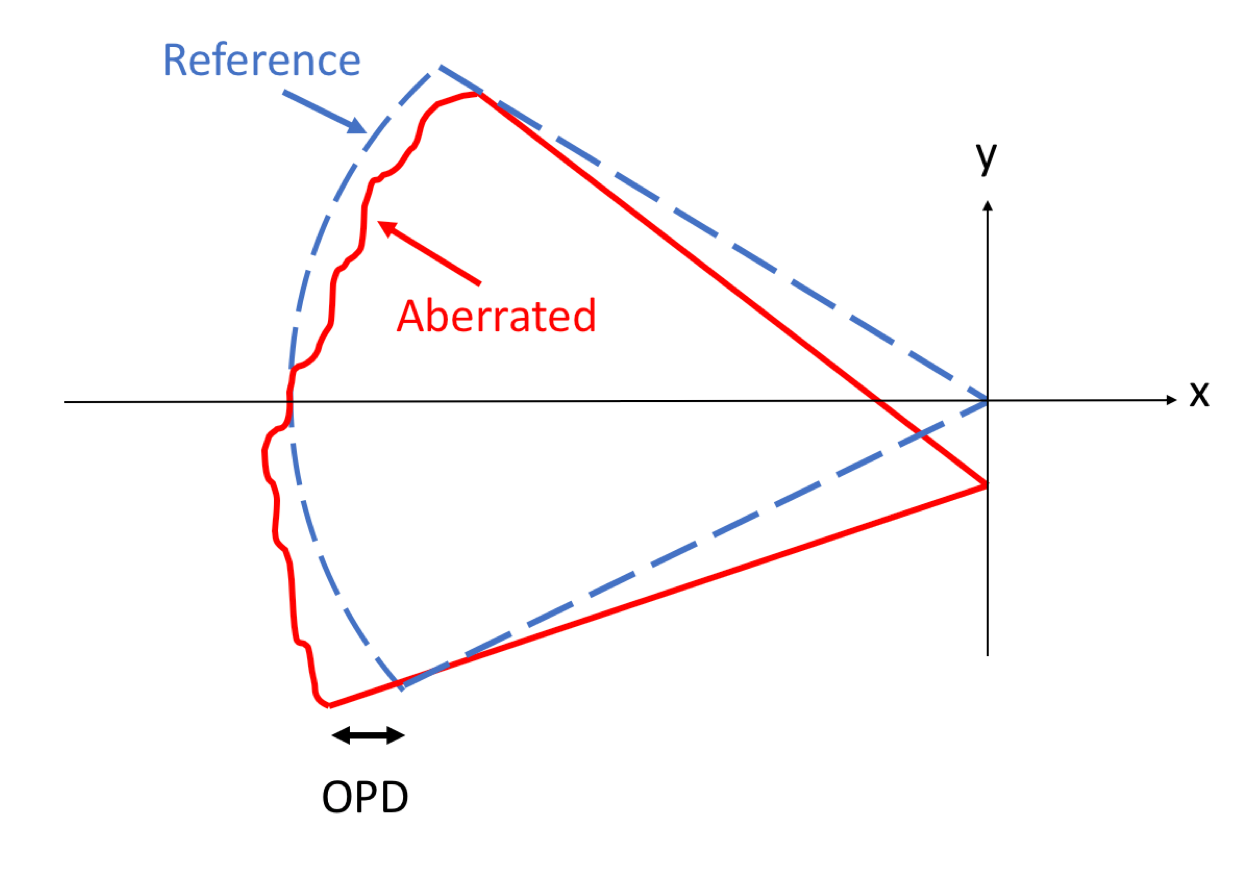
\includegraphics[width=0.75\textwidth]{Chapter Materials/Introduction Materials/Introduction Figures/OPD.png}
    \caption{Caption}
    \label{fig:OPD}
\end{figure}

The Zernike Polynomial generating function is,

\begin{equation}
    \begin{split}
        U_n^m(\rho,\phi)_{even}=R_n^m(\rho)\cos(m\phi) \\
        U_n^m(\rho,\phi)_{odd}=R_n^m(\rho)\sin(m\phi)
    \end{split}
\end{equation}

where $R_n^m(\rho)$ is,

\[ 
R_n^m(\rho)= \left\{
\begin{array}{cr}
       {\sum_{l=0}^{(n-m)/2} \frac{(-1)^l(n-l)!}{l!(\frac{1}{2}(n+m)-l)!(\frac{1}{2}(n-m)-l)!}\rho^{n-2l}} &  \mbox{for n-m even} \\
        {0} &  \mbox{for n-m odd} \\
\end{array} 
\right. 
\]

and $\rho$ and $\phi$ are the radial and azimuthal coordinates, (\cite{weisstein2002zernike}). The first few Zernike polynomials are given in Figure \ref{fig:zernikes}, (\cite{Hsieh:20}). To simulate a phase aberration, a summation of Zernike polynomials weighted by the amplitude is added into the pupil plane as a phase error and the resulting is distorted due to the wavefront error. Examples of the resulting PSF from different Zernike polynomial phase errors is shown in Figure \ref{fig:zernikePSFs}, (\cite{masalehdan2010modeling}).

\begin{figure}[h]
    \centering
    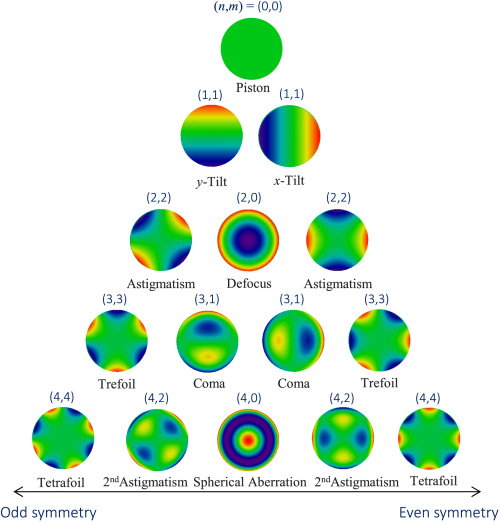
\includegraphics[width=0.5\textwidth]{Chapter Materials/Introduction Materials/Introduction Figures/zernikes.jpeg}
    \caption{First 15 Zernike polynomials.}
    \label{fig:zernikes}
\end{figure}


\begin{figure}
    \centering
    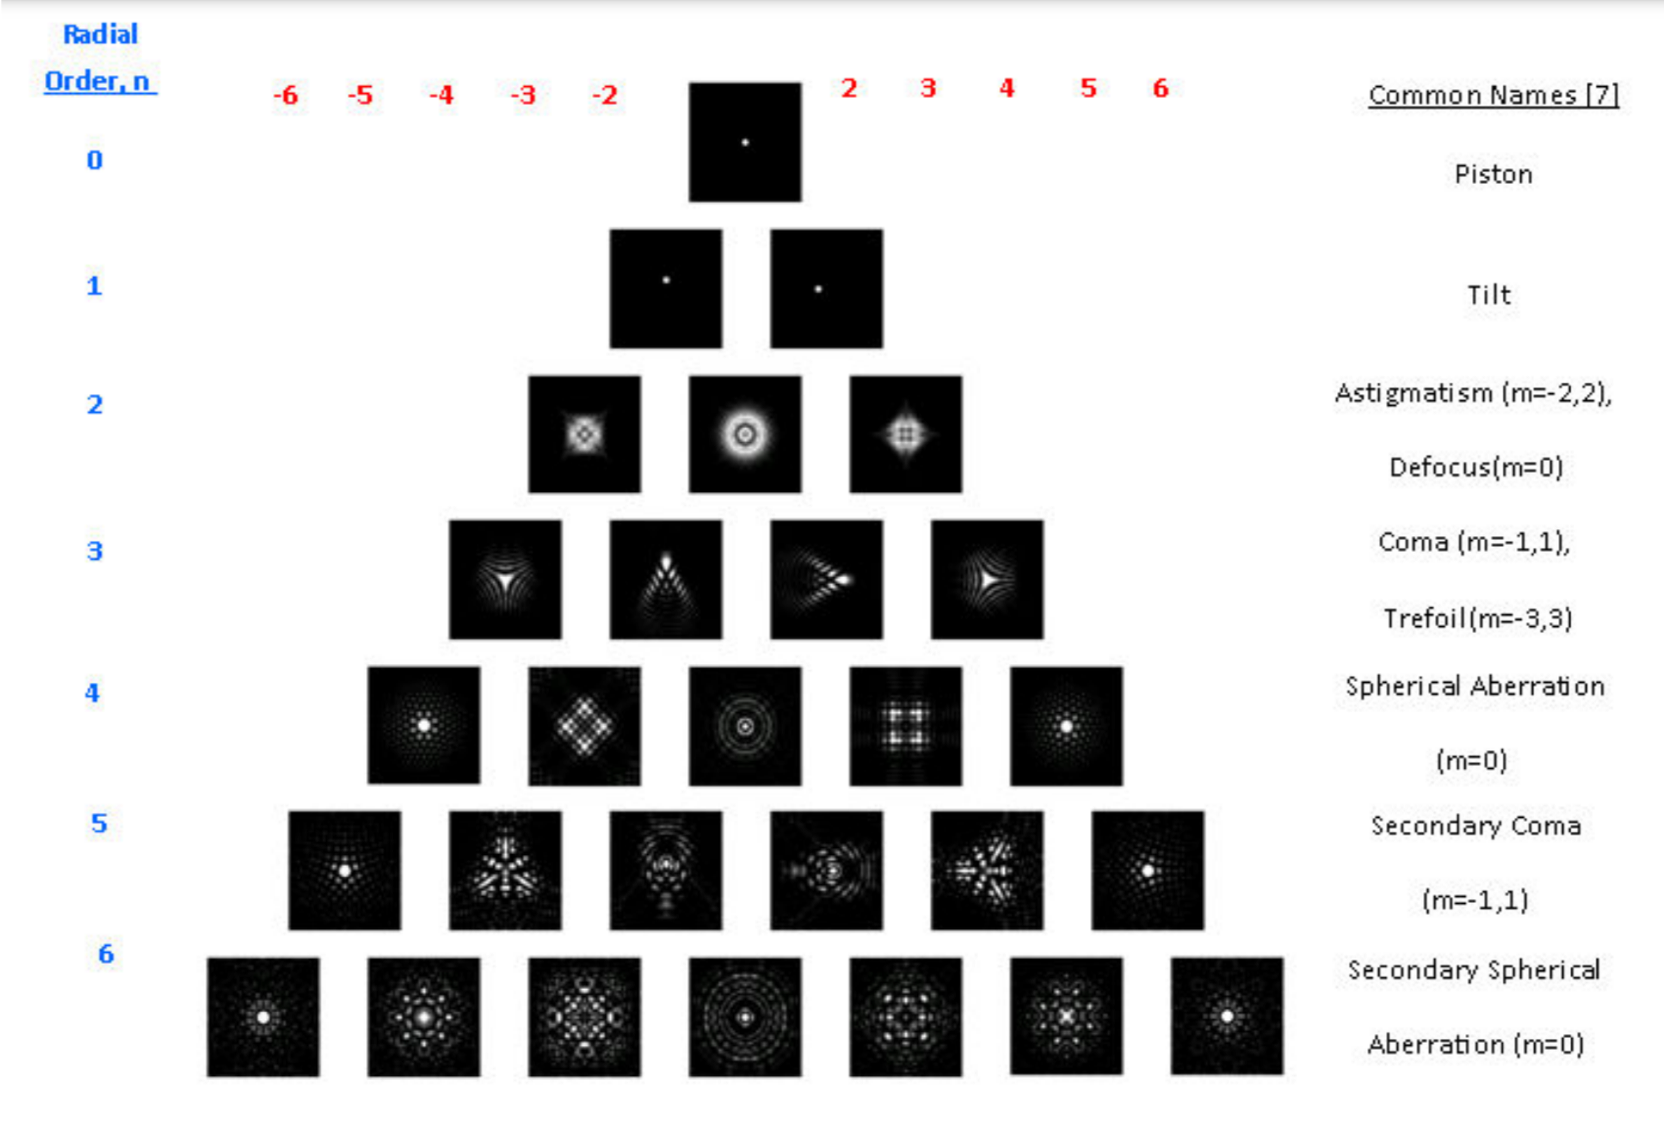
\includegraphics[width=0.75\textwidth]{Chapter Materials/Introduction Materials/Introduction Figures/ZernikePSFs.png}
    \caption{The resulting PSFs from different Zernike modal wavefront errors.}
    \label{fig:zernikePSFs}
\end{figure}

\section{Atmospheric Turbulence}
%%%% 
HARDY CITATION NEEDED


Earth’s atmosphere is divided into layers that have different temperatures. At the boundary between two layers, the temperature gradient causes a shearing effect that results in turbulence. The tropopause that is at a height of about 10-$km$ contributes the largest effect of turbulence on image quality. We describe the structure of atmospheric turbulence using the Kolmogorov model. In this model, the turbulence is described as eddies that have a characteristic outer scale $L_0$ and dissipate heat by breaking into smaller and smaller turbulent cells. Each of these cells has a slightly different index of refraction, and the inhomogeneities in the refractive index impart phase errors on the wavefront. The term $r_0$ is the Fried parameter, and it is defined as the coherence length at which the wavefront error over a circle of radius $r_0$ is 1 radian, (\cite{roddier1999adaptive}). The Fried parameter is used to describe the strength of the distortion imparted by turbulence.  

Turbulence is a statistical process and we are interested in determining the evolution of refractive index at a point $x$ and another point $\Vec{r}$ away. The variance of the difference between the values at these two points is the structure function. The structure function of the refractive index is given by the variance of the refractive index at points $x$ and $x+r$.   

\begin{equation}
    D_N(r)=<|N(x)-N(x,r)|^2>=C_N^2r^{\frac{2}{3}}
\end{equation}

The $C_N^2$ value describes the strength of turbulence as a function of altitude. The $C_N^2$ profile is unique to every observatory because of local topology and climate. The $C_N^2$ profile is used to calculate $r_0$ using:

\begin{equation}
    r_0=[(\frac{2\pi}{\lambda})^2 \int_0^{L_T} C_N^2(z)dz]^{\frac{-3}{5}}
\end{equation}
 
 Where $L_T$ is the total path length of the observation. The Fried parameter scales as a function of wavelength, $r_0 \propto \lambda^{\frac{6}{5}}$, and airmass $r_0 \propto AirMass^{\frac{-5}{3}}$. The seeing $\epsilon$, is a metric used to describe the amount of distortion caused by turbulence at a given wavelength.
 
 \begin{equation}
     \epsilon=\frac{\lambda}{r_0}
 \end{equation}
 
 The mean square wavefront error over a telescope aperture of diameter D due to atmospheric turbulence is calculated using $r_0$.
 
 \begin{equation}
     \sigma^2=1.03(\frac{D}{r_0})^{\frac{5}{3}}
 \end{equation}


Atmospheric turbulence does not impart equally strong phase errors across all spatial frequencies. The distribution of power imparted by atmospheric turbulence to different spatial scales is described by the Kolmogorov power spectrum, which is given by Equation \ref{Power}\cite{rampy2012production}. The power spectrum relates the strength of an aberration at a given spatial frequency, $k$, to the seeing conditions, $r_0$. The phase errors imparted by atmospheric turbulence are strongest at low spatial frequencies.

\begin{equation}
    P(k)=0.027r_0^{-5/3}k^{-11/3}
    \label{Power}
\end{equation}



The effect of atmospheric turbulence is to lower the resolution of the optical system. For a long exposure image, the image is a disk with an angular FWHM of $\approx \frac{\lambda}{r_0 }$. For short exposure images, we expect a speckle pattern of approximately $\frac{D}{r_0}$ speckles of width equal to the diffraction limit of the system. For a system partially corrected for by adaptive optics, the PSF is a diffraction-limited peak surrounded by the residual uncorrected $\frac{D}{r_0}$ halo. Figure \ref{fig:turbPSF} shows a time-averaged closed-loop PSF.

\begin{figure}
    \centering
    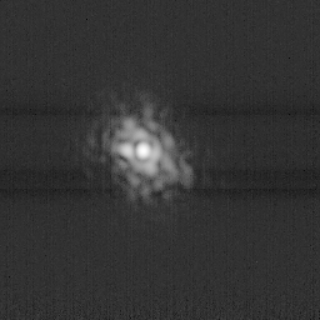
\includegraphics{Chapter Materials/Chapter One Materials/turbPSF.png}
    \caption{Image of a time-averaged PSF. The Airy pattern can be seen in the center of the disk that is the result of uncorrected phase error.}
    \label{fig:turbPSF}
\end{figure}


 \section{Introduction to Adaptive Optics}
 
%Adaptive optics systems correct for the blurring of Earth's atmosphere in real time.

In astronomy there are different types of adaptive optics systems developed to maximize correction for different objects. Ground Layer Adaptive Optics (GLAO) systems such as ARGOS (\cite{rabien2019argos}) at the LBT, and 'Imaka (\cite{abdurrahman2018improved}) at the University of Hawaii 2.2 meter telescope compensate ground layer turbulence to produce a uniform correction across a greater than 1 arcmin field of view. Multi-conjugate Adaptive Optics (MCAO) systems such as the Gemini Multi-conjugate Adaptive Optics System (\cite{neichel2014gemini}) have multiple deformable mirrors and wavefront sensors conjugated to layers of atmospheric turbulence at different altitudes. MCAO systems provide well corrected PSFs over a large field of view. Extreme adaptive optics systems (ExAO) are adaptive optics systems optimized for excellent wavefront correction of an on-axis guide star at the spatial frequencies of the high-contrast region of a coronagraph. 

Adaptive optics systems operate under the concept of conjugate imaging. Figure \ref{fig:AOdiagram} shows the overview of the optical path of an AO system. Light from the guide star travels through the layers of Earth's atmosphere and acquires phase errors from atmospheric turbulence. In single conjugate AO we model the effects of atmospheric turbulence as a single phase screen at a known altitude that imparts all of the phase errors to the guide star's wavefront. This layer of turbulence is typically modeled to be in the entrance pupil and is imaged to conjugate planes in the AO system. The optical design of an AO system consists primarily of pupil relays that re-size and re-image the pupil plane onto the wavefront sensor and DM so that the turbulence screen is both sensed and corrected in the same plane. Adaptive optics systems work over a wavelength bandpass; to mitigate the effect of chromatic aberrations through the system mirrors are used as the optics in these pupil relays. In a closed loop AO system the wavefront sensor is placed after the DM. When the loop is closed the wavefront sensor sees a wavefront that is the combination of the atmospheric turbulence and the correction applied to the DM. There is a time lag between when the wavefront is sensed and when the correction applied which results in uncorrected wavefront errors that are quantified by the temporal error in the AO error budget. ExAO systems are designed to be low latency and run at loop speeds greater than 1-kHz.




\begin{figure}
    \centering
    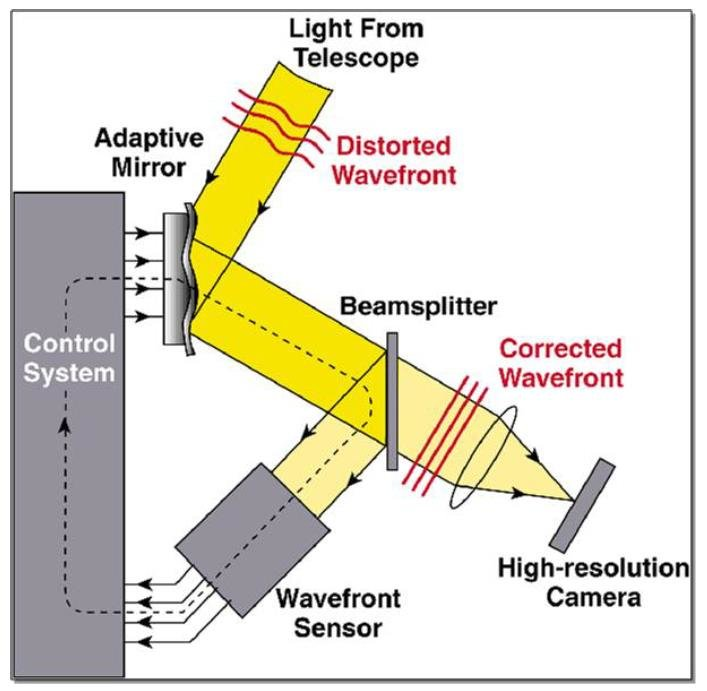
\includegraphics[width=0.8\textwidth]{Chapter Materials/Chapter Two Materials/Adaptive-Optics-System.png}
    \caption{Diagram of an adaptive optics closed loop,(\cite{suarez2017approach}). Light from the telescope is first read into the wavefront sensor. A control system uses that signal to compute the commands to drive the deformable into the shape that will correct the wavefront. The result is a corrected wavefront.}
    \label{fig:AOdiagram}
\end{figure}

There are several ExAO instruments in operation on current generation telescopes. Current instruments include the Subaru Coronagraphic Extreme Adaptive Optics instrument (SCExAO)\cite{jovanovic2015subaru}, the Spectro-Polarimetric High-contrast Exoplanet Research instrument (SPHERE)\cite{beuzit2008sphere}, the Gemini Planet Imager (GPI)\cite{macintosh2014first}, the Keck Planet Imager and Characterizer (KPIC)\cite{jovanovic2019keck}, and most recently the Magellan Extreme Adaptive Optics System (MagAO-X)\cite{males2020magao}. All of these instruments have common features: a high actuator count deformable mirror running at extreme speeds (at least 1kHz), a high-performance wavefront sensor (WFS), and a high-contrast coronagraph These instruments are pathfinders for ExAO systems on the GSMTs.






% Wavefront sensors have different sensitivities to phase errors of different spatial frequencies. In ExAO we need a wavefront sensor that is highly sensitive across all spatial frequencies to maximize light suppression by the coronagraph, and reduce high spatial frequency speckle noise in short exposure images. In an ideal adaptive optics system the dominating source of noise on the wavefront sensor measurement is photon noise. The value $\beta_p$ is used quantify the sensitivity to photon noise of a wavefront sensor. Figure \ref{fig:guyon2005} plots $\beta_p$ as a function of spatial frequency for different types of wavefront sensors. The most sensitive wavefront sensor is the Zernike wavefront sensor (ZWFS), that has a $\beta_p=1$ across all spatial frequencies, and the unmodulated pyramid wavefront sensor (FPYRWFS) is a close second with a $\beta_p=\sqrt{2}$ at all spatial frequencies. These wavefront sensors suffer from a lack of dynamic range. Phase errors from the turbulent atmosphere vary in strength, and large phase errors cause the signals from the Zernike and Pyramid wavefront sensors to become nonlinear. The pyramid wavefront sensor has the option of modulation which increases the linearity of signal at the cost of sensitivity. The ability to balance the sensitivity and dynamic range with the pyramid makes it robust to different seeing conditions and is ideal for ExAO wavefront sensing. 









\subsection{The Strehl Ratio}

INCLUDE A FIGURE

An adaptive optics system compensates phase errors to return the resolution of the system to the diffraction limit of the telescope. The correction is not perfect, and we are interested in measuring the performance of the AO system. The Strehl ratio is defined as the ratio between the peak of an imaged PSF, with the peak of an aberration-free PSF. The Strehl ratio can be used to approximate the residual RMS uncorrected phase errors through the Marechal approximation given by:

\begin{equation}
    S \cong e^{-\sigma^2}
\end{equation}

where $S$ is the Strehl ratio, and $\sigma^2$ is the phase variance of the wavefront in units of radians. The measurement of the Strehl ratio for an AO corrected PSF is given in Equation \ref{Strehl}. The Strehl ratio is calculated by taking the ratio of the peak intensity of the partially corrected PSF, $P_{data}$,  to the peak intensity of an aberration free PSF, $P_0$. The peaks are normalized by the flux in the image. A simulated model can be used for the aberration free image. 


\begin{equation}
    S=\frac{P_{data}/Flux_{data}}{P_{0}/Flux_{0}}
    \label{Strehl}
\end{equation}



